% Baccalauréat malgache, série C, 2013 : énoncé.
\TCDBacAttribution{C}{2013}
\providecommand{\dx}{\mathrm{d}x}
\providecommand{\Re}[1]{\mathrm{Re}\left( #1 \right)}
\providecommand{\Im}[1]{\mathrm{Im}\left( #1 \right)}
\providecommand{\dt}{\mathrm{d}t}
%
%%%%%%%%%%%%%%%%%%%%%%%%%%%%%%%%%%%%%%%%%%%%%%%%%%%%%%%%%%%%%%%%%%%%%%%%%%%%%%%%%%%%%%%%%%%%%%%%%%%%%%%%%%%%%%%%%%%%%%%%%%%%%%%%
\noindent \underline{\textsc{\textbf{Exercice}}} (4 points) \\[-1\baselineskip]
%
      \begin{description}
            \item[A.] \underline{Arithm\'etique} \newline
                  \begin{enumerate}
                        \item Un nombre $A$ s'\'ecrit $121$ en base $4$ et 
                              $221$ en base $n$, $n\in\mathbb{N}^*$. D\'eterminer $n$.
                        \item Prouver que pour tout entier naturel $n$, 
                              $2^{5n+1} + 9^{n+1} \equiv 0 [11]$.
                        \item R\'esoudre dans $\mathbb{N}\times\mathbb{N}$ le syst\`eme
                              $\begin{multiform} PGCD(a;b) = 6 \\ PPCM(a;b) = 240 \end{multiform}$.
                  \end{enumerate}
            \item[B.] \underline{Probabilit\'e} \newline
                  $n\in\mathbb{N}^*$.
                  On dispose de $n$ boules num\'erot\'ees de $1$ \`a $n$.
                  On veut placer ces boules dans $n$ bo\^ites num\'erot\'ees de $1$ \`a $n$ ;
                  chacune des bo\^ites pouvant contenir de $0$ \`a $n$ boules.
                  \begin{enumerate}
                        \item Pour $n=4$, calculer la probabilit\'e des \'ev\`enements suivants :
                              \begin{description}
                                    \item[E :] << Chaque bo\^ite contient une boule >>.
                                    \item[F :] << Chaque bo\^ite contient une boule de telle sorte que la bo\^ite et la boule ont le m\^eme num\'ero >>.
                                    \item[G :] << La bo\^ite num\'erot\'ee $1$ contient exactement deux boules >>.
                              \end{description}
                        \item Pour $n\geq 2$, on d\'esigne par $P_n(k)$ la probabilit\'e pour que 
                              la bo\^ite num\'erot\'ee $1$ contienne exactement $k$ boule(s), $k\in\{ 0,1,2,\ldots,n\}$.
                              \begin{enumerate}
                                    \item D\'emontrer que, pour tout $n$, 
                                          $P_n(k) = C_n^k \left(\frac{1}{n}\right)^k \left( 1 - \frac{1}{n} \right)^{n-k}$.
                                    \item En d\'eduire que : 
                                          $\sum_{k=0}^n C_n^k (n-1)^{n-k} = n^n$.
                              \end{enumerate}
                  \end{enumerate}
      \end{description}
%%%%%%%%%%%%%%%%%%%%%%%%%%%%%%%%%%%%%%%%%%%%%%%%%%%%%%%%%%%%%%%%%%%%%%%%%%%%%%%%%%%%%%%%%%%%%%%%%%%%%%%%%%%%%%%%%%%%%%%%%%%%%%%%
\noindent \underline{\textsc{\textbf{PROBLEME I}}} (7 points) \newline
%
      \underline{\textbf{NB :}} Les parties A et B sont ind\'ependantes.

      \underline{\textbf{Partie A}} \newline
            \begin{minipage}{0.3\actualtextwidth}
                  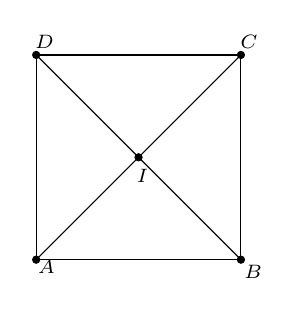
\begin{tikzpicture}[x=.65cm,y=.65cm]
                  \draw (-2,-2)-- (2,-2);
                  \draw (2,-2)-- (2,2);
                  \draw (2,2)-- (-2,2);
                  \draw (-2,2)-- (-2,-2);
                  \draw (2,-2)-- (-2,2);
                  \draw (-2,-2)-- (2,2);
                  \begin{scriptsize}
                  \fill [color=black] (-2,-2) circle (1.5pt);
                  \draw[color=black] (-1.8,-2.14) node {$A$};
                  \fill [color=black] (2,-2) circle (1.5pt);
                  \draw[color=black] (2.24,-2.24) node {$B$};
                  \fill [color=black] (2,2) circle (1.5pt);
                  \draw[color=black] (2.16,2.26) node {$C$};
                  \fill [color=black] (-2,2) circle (1.5pt);
                  \draw[color=black] (-1.84,2.26) node {$D$};
                  \fill [color=black] (0,0) circle (1.5pt);
                  \draw[color=black] (0.08,-0.36) node {$I$};
                  \end{scriptsize}
                  \end{tikzpicture}
            \end{minipage}
            %
            \begin{minipage}{.65\actualtextwidth}
                  Dans le plan complexe $\mathscr{P}$, on consid\`ere le carr\'e direct $ABCD$ de centre $I$.
                  Quels que soient les points $M$ et $N$ du plan, on note par :
                        \begin{itemize}
                              \item $r_M$ la rotation de centre $M$ et d'angle $\frac{\pi}{2}$.
                              \item $t_{\overrightarrow{MN}}$ la translation de vecteur $\overrightarrow{MN}$.
                              \item $\mathscr{S}_{(MN)}$ la r\'eflexion d'axe $(MN)$.
                        \end{itemize}
            \end{minipage}
            %
            \begin{enumerate}
                  \item En d\'ecomposant $r_A$ et $r_B$, d\'eterminer la nature et les \'el\'ements g\'eom\'etriques de $r_B \circ r_A$.
                  \item Le plan $\mathscr{P}$ est rapport\'e au rep\`ere orthonormal $R = (A ; \vec{u} , \vec{v})$ o\`u $\vec{u} = \overrightarrow{AB}$ et $\vec{v} = \overrightarrow{AD}$.
                        \begin{enumerate}
                              \item D\'eterminer la forme alg\'ebrique de $a=\frac{z_A - z_C}{z_B - z_C}$.
                              \item En d\'eduire l'angle et le rapport de la similitude plane directe de centre $C$ qui transforme $B$ en $A$.
                        \end{enumerate}
                  \item Soit $f = \mathscr{S}_{(AD)} \circ r_A \circ t_{\overrightarrow{AC}}$.
                        \begin{enumerate}
                              \item D\'emontrer que $f$ est un antid\'eplacement.
                              \item En d\'ecomposant convenablement $r_A$, pr\'eciser la nature et les \'el\'ements caract\'eristiques de $f$.
                              \item En d\'eduire l'expression complexe de $f$.
                        \end{enumerate}
            \end{enumerate}
      
      \underline{\textbf{Partie B}} \newline
            \begin{enumerate}
                  \item Etant donn\'e un nombre r\'eel $\theta$.
                        R\'esoudre dans $\mathbb{C}$ l'\'equation \`a variable $t$,
                        $(E_\theta) : t^2 - 2t \; \cos \theta + 1 = 0$.
                        En d\'eduire les solutions dans $\mathbb{C}$ de l'\'equation \`a variable complexe $z$, $(E_\theta ') : z^4 - 2z^2 \; \cos \theta + 1 = 0$.
                  \item On d\'esigne par $A$, $B$, $C$ et $D$ les images des solutions de 
                        l'\'equation $\left( E'_{\frac{\pi}{3}} \right)$ telles que : 
                        $ \Re{z_A} < 0 $ ; $ \Im{z_B} < 0 $ avec $z_B = -z_A$ ; 
                        $z_D = \bar{z}_A$ et $z_C = \bar{z}_B$ o\`u $z_A$, $z_B$, $z_C$ et $z_D$ sont 
                        les affixes respectives des points $A$, $B$, $C$ et $D$.
                        \begin{enumerate}
                              \item Placer les points $A$, $B$, $C$ et $D$ sur le cercle trigonom\'etrique d'unit\'e 3~cm. 
                                    \label{quest:2/a)}
                              \item Pour quelle valeur de $\theta$ les points $A$, $B$, $C$ et $D$ sont-ils les sommets d'un carr\'e\,?
                        \end{enumerate}
                  \item $A$, $B$, $C$ et $D$ \'etant les sommets du rectangle d\'efini dans la question \ref{quest:2/a)} 
                        et $\lambda$ un r\'eel tel que $\lambda \in [-1 ; 1]$.
                        On appelle $G_\lambda$ le barycentre du syst\`eme des points pond\'er\'es
                        $S_\lambda = \left\lbrace (A ; \lambda^2 + 1) ; (B ; \lambda) ; (D ; -\lambda) \right\rbrace$.
                        \begin{enumerate}
                              \item Exprimer $\overrightarrow{AG_\lambda}$ en fonction de $\overrightarrow{BD}$.
                              \item On pose 
                              		$\scriptstyle{(E) = \left\lbrace 
                                    M \in \mathscr{P} \text{ tel que } 
                                    \left\| 2\overrightarrow{MA}+\overrightarrow{MB}-\overrightarrow{MD} \right\|
                                    = \left\| 2\overrightarrow{MA}-\overrightarrow{MB}+\overrightarrow{MD} \right\|
                                    \right\rbrace}$.
                                    D\'eterminer et construire $(E)$.
                        \end{enumerate}
            \end{enumerate}

%%%%%%%%%%%%%%%%%%%%%%%%%%%%%%%%%%%%%%%%%%%%%%%%%%%%%%%%%%%%%%%%%%%%%%%%%%%%%%%%%%%%%%%%%%%%%%%%%%%%%%%%%%%%%%%%%%%%%%%%%%%%%%%%
\noindent \underline{\textsc{\textbf{PROBLEME II}}} (9 points) \newline
%
      Soit $f$ la fonction d\'efinie sur l'intervalle $]0 ; +\infty[$ par :
      \[
            \begin{multiform}
                  f(x) = x^2 - 1 - 2\ln x  \text{ si }  x \in\ ]0 ; 1[ \\
                  f(x) = (3x-3) \expo{-x}  \text{ si }  x \geq 1      \;.
            \end{multiform}
      \]
      On note par $(C)$ sa courbe dans un rep\`ere orthonorm\'e d'unit\'e graphique 4~cm.
      
      \underline{\textbf{Partie A}} %\newline
            \begin{enumerate}
                  \item \begin{enumerate}
                              \item D\'emontrer que $f$ est continue au point d'abscisse $1$.
                              \item Etudier la d\'erivabilit\'e de $f$ au point d'abscisse $1$.
                        \end{enumerate}
                  \item \begin{enumerate}
                              \item Etudier, suivant les valeurs de $x$, le sens de variation de $f$.
                              \item Dresser alors le tableau de variation de $f$.
                        \end{enumerate}
                  \item \begin{enumerate}
                              \item D\'emontrer que $f$ admet un unique point d'inflexion $I$ que l'on d\'eterminera.
                              \item D\'eterminer l'\'equation de la tangente $(T)$ \`a $(C)$ au point $I$.
                              \item Tracer $(T)$ et $(C)$ dans le m\^eme rep\`ere 
                                    en pr\'ecisant les demi-tangentes au point d'abscisse $1$.
                        \end{enumerate}
            \end{enumerate}
            
            
      \underline{\textbf{Partie B}} \newline
            Pour tout r\'eel $\lambda$ tel que $0 < \lambda < 1$, on pose $I(\lambda) = \int_{\lambda}^{1} f(t) \dt$.
            Quels que soient les entiers $n$ et $k$ tels que : $n \geq 2$ et $1 \leq k \leq n-1$, on pose
            $\displaystyle{S_n = \frac{1}{n} \sum_{k=1}^{n} f\left( \frac{k}{n} \right)}$.
            \begin{enumerate}
                  \item \begin{enumerate}
                              \item A l'aide d'une int\'egration par parties, d\'eterminer $I(\lambda)$ en fonction de $\lambda$.
                              \item Calculer $\displaystyle{\lim_{\lambda \rightarrow 0} I(\lambda)}$.
                        \end{enumerate}
                  \item \begin{enumerate}
                              \item D\'emontrer que 
                                    $\displaystyle{ 
                                                     \frac{1}{n} f\left( \frac{k+1}{n} \right) 
                                                           \leq 
                                                     \int_{\frac{k}{n}}^{\frac{k+1}{n}} f(t) \dt
                                                           \leq 
                                                     \frac{1}{n} f\left( \frac{k}{n} \right)
                                                       }$.
                              \item En d\'eduire que
                                    $\displaystyle{
                                                     \frac{1}{n} \sum_{k=2}^{n} f\left( \frac{k}{n} \right) 
                                                           \leq 
                                                     \int_{\frac{1}{n}}^{\frac{1}{n}} f(t) \dt
                                                           \leq 
                                                     \frac{1}{n} \sum_{k=1}^{n-1} f\left( \frac{k}{n} \right)
                                                       }$.
                              \item D\'emontrer alors que 
                                    $\displaystyle{
                                                     I\left( \frac{1}{n} \right)
                                                           \leq 
                                                     S_n
                                                           \leq 
                                                     I\left( \right) + \frac{1}{n} f\left(\frac{1}{n}\right)
                                                       }$.
                              \item D\'eterminer $\displaystyle{\lim_{t\rightarrow0} t f(t)}$.
                              \item Calculer ainsi $\displaystyle{\lim_{n\rightarrow+\infty} S_n}$.
                        \end{enumerate}
            \end{enumerate}
      \underline{\textbf{NB :}} Pour la construction, on prend $\expo{-1} = 0,4$ ; $\expo{-2} = 0,2$ et $\expo{-3} = 0,05$.
%%%%%%%%%%%%%%%%%%%%%%%%%%%%%%%%%%%%%%%%%%%%%%%%%%%%%%%%%%%%%%%%%%%%%%%%%%%%%%%%%%%%%%%%%%%%%%%%%%%%%%%%%%%%%%%%%%%%%%%%%%%%%%%%




































